\documentclass[a4paper, 12pt]{article}

\usepackage{lmodern} % Police standard sous LaTeX : Latin
\usepackage[french]{babel} % Pour la langue francaise
\usepackage[utf8]{inputenc} % Pour l'UTF-8
\usepackage[T1]{fontenc} % Pour les césures des caractères
\usepackage{graphicx}
\usepackage{subfig}
\usepackage{ragged2e}
\justifying

\renewcommand{\thesection}{\Alph{section}}

\title{Modèle de diffusion d'une maladie dans une population d'agents mobiles}
\author{NIDDAM Benjamin}
\date{\today}

\begin{document}
\begin{titlepage}
	\maketitle
\end{titlepage}

\newpage

\tableofcontents

\newpage

\section{Présentation du modèle}
\subsection{Définition des variables}

\subsection{Présentation des agents}

\subsection{Définition des intéractions}


\newpage
\section{Exprériences, résultats et limites}
\subsection{État initial}

Dans toutes nos simulations nous utilisons un nombre d'agents fixé à 1000, un nombre d'agents contaminés au temps zéro fixé à 1 puis à 100 et un degré de contamination à 3.5\%.

Avant de commencer les tests pour endiguer la maladie, nous avons simuler l'évolution de celle-ci sans mesures de restrictions. Voici les résultats obtenus:

\begin{figure}[!h]
	\centering
	\subfloat[\centering 1 agents contaminés à t0]{{\includegraphics[width=6cm]{../Courbes/1000_agents_1_contaminé_5_ans/Natural_immunity_only.png} }}
	\qquad
	\subfloat[\centering 100 agents contaminés à t0]{{\includegraphics[width=6cm]{../Courbes/1000_agents_100_contaminé_5_ans/Natural_immunity_only.png} }}
	\caption{Représentations graphique de l'évolution de l'état\\ de la population en fonction du temps}

\end{figure}

On observe des vagues de guérisons et de contaminations qui s'étendent jusqu'à la fin de la simulation. Ces
vagues sont dues au fait que nos agents obtiennent une immunité naturelle temporaire après chaque
guérison.

\vspace{0.8cm}

Nous avons mit en place plusieurs expériences pour tenter de ralentir ou d'éradiquer la maladie. Pour chaque
expérience, nous avons conserver les mêmes paramètres pour la simulation et réitéré 5 fois. Nous utilisons la
moyenne des valeurs obtenues dans ces simulations pour réduire les incertitudes dues à l'aléatoire

\newpage

\subsection{Confinement}
Comme première expérience nous avons décidé de confiner la population. Pour ce faire nous divisons les
valeurs de vx et vy par deux, puis par trois et enfin par cinq. Ce qui nous ramène à trois tests que nous
appelons respectivement "confinement léger", "confinement moyen" et "confinement strict" par rapport à leur
taux de limitation. Ce taux fera baisser la possibilité de déplacement des agents jusqu'à la quasi-immobilité
lorsque ce dernier vaut cinq. Ceci entraine donc une réduction des interactions entre les agents qui devrait
limiter la dispersion de la maladie. On veut savoir si cette réduction est suffisante pour éradiquer la maladie. Et
si oui, quel taux faut-il mettre en place et sûr combien de temps. Nous avons donc réalisé les simulations
suivantes:

\begin{figure}[!h]
	\centering
	\subfloat[\centering Light confinement]{{\includegraphics[width=6cm]{../Courbes/1000_agents_1_contaminé_5_ans/Light_confinement.png} }}
	\qquad
	\subfloat[\centering Basic confinement]{{\includegraphics[width=6cm]{../Courbes/1000_agents_1_contaminé_5_ans/Partial_confinement.png} }}
	\centering
	\subfloat[\centering Heavy confinement]{{\includegraphics[width=6cm]{../Courbes/1000_agents_1_contaminé_5_ans/Natural_immunity_only.png} }}
	\qquad
	\caption{Représentations graphique de l'évolution de l'état\\ de la population en fonction du taux de confinement}

\end{figure}

\newpage

Les graphiques ci-dessus représentent l'évolution de l'état des agents au cours de la simulation (temps en jour)en fonction du taux de confinement.
On observe que la méthode de confinement est une facon très efficace de ralentir le déplacement de la maladie au sein de la population. On le constate clairement
sur les graphiques du confinement léger et moyen. En effet, le pic de contamination initial est beaucoup moins important que celui de la simulation sans restrictions.
Enfin, en se basant sur la courbe du confinement stricte, on confirme que cette méthode, malgré un degré très important de limitations, n'est pas suffisante pour éradiquer la maladie.
On peut donc envisager de combiner cette dernière avec une autre méthode. Mais avant cela, nous avons testé si mettre en place un confinement de la population alors que la s'est déja bien propagé.
Nous obtenons donc le résultat suivant:

\begin{figure}[!h]
	\centering
	\subfloat[\centering Light confinement]{{\includegraphics[width=6cm]{../Courbes/1000_agents_100_contaminé_5_ans/Light_confinement.png} }}
	\qquad
	\subfloat[\centering Basic confinement]{{\includegraphics[width=6cm]{../Courbes/1000_agents_100_contaminé_5_ans/Partial_confinement.png} }}
	\centering
	\subfloat[\centering Heavy confinement]{{\includegraphics[width=6cm]{../Courbes/1000_agents_100_contaminé_5_ans/Strict_confinement.png} }}
	\qquad
	\caption{Représentations graphique de l'évolution de l'état\\ de la population en fonction du taux de confinement}

\end{figure}

\newpage

\subsection{Respect des gestes barrières}
Dans un deuxième temps, nous avons décidé de mettre en place un respect des gestes barrières. Cette méthode cherche à réduire la probabilité qu'un agent contaminé transmette la maladie à un autre agent
lors de leur rencontre. Pour ce faire, nous avons mit en place trois intensités: "Basics barrier gestures", "Mediums barrier gestures" et "Heavys barrier gestures" qui réduisent par deux, trois et cinq
la probabilité d'infection. Dans ce cas, on veut savoir jusqu'à quel niveau les gestes barrières peuvent ralentir la maladie.

\begin{figure}[!h]
	\centering
	\subfloat[\centering Light confinement]{{\includegraphics[width=6cm]{../Courbes/1000_agents_1_contaminé_5_ans/Light_confinement.png} }}
	\qquad
	\subfloat[\centering Basic confinement]{{\includegraphics[width=6cm]{../Courbes/1000_agents_1_contaminé_5_ans/Partial_confinement.png} }}
	\centering
	\subfloat[\centering Heavy confinement]{{\includegraphics[width=6cm]{../Courbes/1000_agents_1_contaminé_5_ans/Strict_confinement.png} }}
	\qquad
	\caption{Représentations graphique de l'évolution de l'état\\ de la population en fonction du taux de gestes barrières}

\end{figure}

\newpage

Ici, nous représentons l'évolution de l'état des agents au fil du temps (en jour) en fonction du degrés de respect de la population pour les gestes barrières.
On voit clairement que les gestes barrières sont très efficaces pour réduire la transmission de la maladie même si les agents ne les suivent pas de manière stricte comme le montre le graphique
"gestes barrières basiques". Grace au courbes, il est clair que les gestes barrières sont une très bonne
pratique pour réduire la transmission de la maladie. De plus, comme le montre le graphique"gestes barrières strictes", si respectés sérieusement et dès les premiers jours, une épidémie peut facilement
être évitée. Mais on peut aussi se demander si cette méthode serait aussi utile, si mise en place alors que l'épidémie est déjà en cours. Voici donc les résultats obtenus pour ce cas:

\begin{figure}[!h]
	\centering
	\subfloat[\centering Light confinement]{{\includegraphics[width=6cm]{../Courbes/1000_agents_100_contaminé_5_ans/Light_confinement.png} }}
	\qquad
	\subfloat[\centering Basic confinement]{{\includegraphics[width=6cm]{../Courbes/1000_agents_100_contaminé_5_ans/Partial_confinement.png} }}
	\centering
	\subfloat[\centering Heavy confinement]{{\includegraphics[width=6cm]{../Courbes/1000_agents_100_contaminé_5_ans/Strict_confinement.png} }}
	\qquad
	\caption{Représentations graphique de l'évolution de l'état\\ de la population en fonction du taux de confinement}

\end{figure}

\newpage

Dans le cas présent, le développement de la maladie est atténué par les gestes barrières. Cependant, comme pour l'expérience précédente, à part lorsque les gestes barrières sont fortement respectés, 
l'épdiémie n'est pas évitée.

\newpage

\subsection{Vaccination}

Nous avons ensuite instauré un cycle de vaccination. En effet, dans la simulation, chaque jour, nous vaccinons un nombre d'agents définits au préalable.Le vaccin donne une imunité plus longue que celle obtenue 
naturellement. Au seins même de cette expérience nous avons pu tester plusieurs choses. Dans un premier temps, les agents n'effectuent qu'une seule vaccination qui les imunisent un certain temps mais finissent 
par attraper la maladie à la fin de leur prériode de vaccination.

\begin{figure}[!h]
	\centering
	\subfloat[\centering 1 vaccination par jour]{{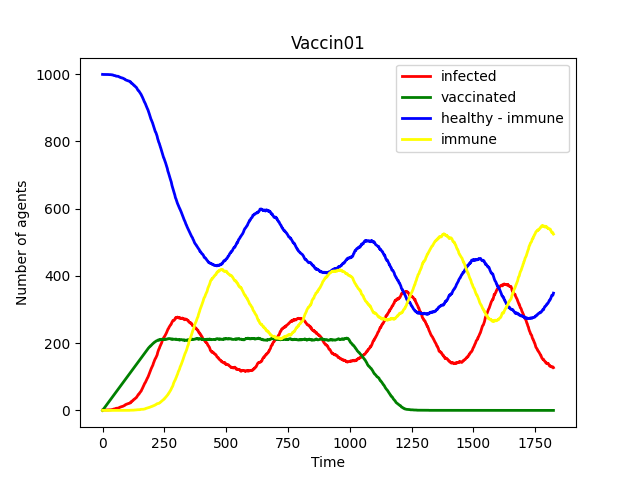
\includegraphics[width=6cm]{../Courbes/1000_agents_1_contaminé_5_ans/Vaccin01.png} }}
	\qquad
	\subfloat[\centering 3 vaccination par jour]{{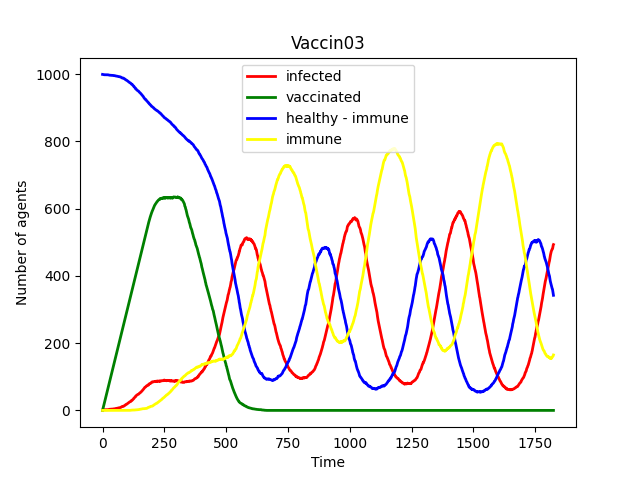
\includegraphics[width=6cm]{../Courbes/1000_agents_1_contaminé_5_ans/Vaccin03.png} }}
	\centering
	\subfloat[\centering 4 vaccination par jour]{{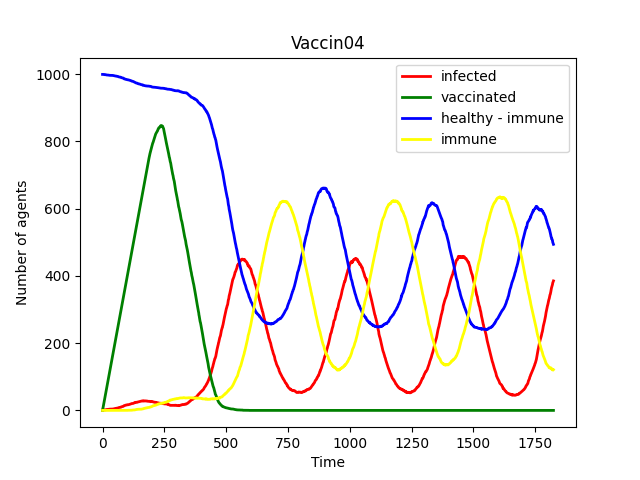
\includegraphics[width=6cm]{../Courbes/1000_agents_1_contaminé_5_ans/Vaccin04.png} }}
	\qquad
	\caption{Représentations graphique de l'évolution de l'état\\ de la population en fonction du nombre de nouveaux vaccinés par jours}

\end{figure}

C'est graphiques représentent l'évolution de l'état de la population en fonction du temps (en jours) pour un nombre de personnes qui se font vacciner chaque jour.
On observe que le fait d'avoir une partie de la population vaccinée est une bonne pratique pour réduire la transmission de la maladie. En effet, le pic de vaccination permet de
fortement retardé le pic de contamination initial.
\newpage
De plus, on peut voir que nombre de personnes qui se vaccinent chaque jour est un facteur important pour retarder le début de l'épidémie.

Par la suite, nous avons implémenté les rappels de vaccins. Nous revaccinons les agents dès lors que leur vaccin ne fait plus effet. On regarde donc le seuil minimal de personnes à vacciner par jour
pour que la maladie soit éradiquée.

\begin{figure}[!h]
	\centering
	\subfloat[\centering 1 vaccination par jour]{{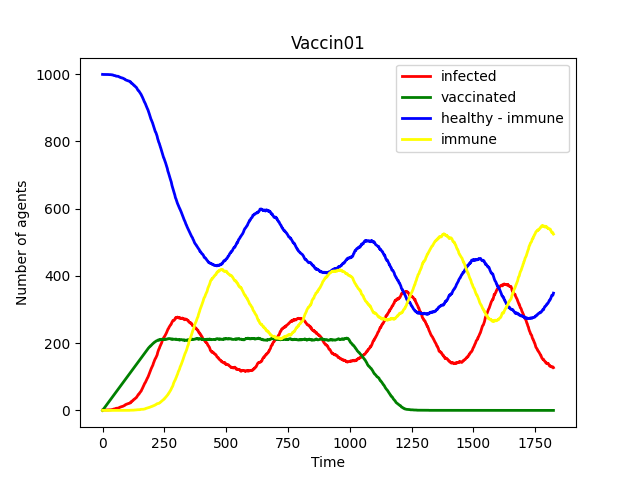
\includegraphics[width=6cm]{../Courbes/1000_agents_1_contaminé_5_ans/Vaccin01.png} }}
	\qquad
	\subfloat[\centering 3 vaccination par jour]{{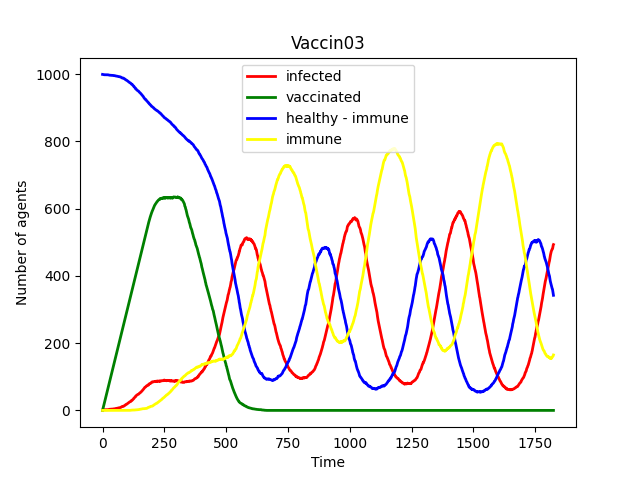
\includegraphics[width=6cm]{../Courbes/1000_agents_1_contaminé_5_ans/Vaccin03.png} }}
	\centering
	\subfloat[\centering 4 vaccination par jour]{{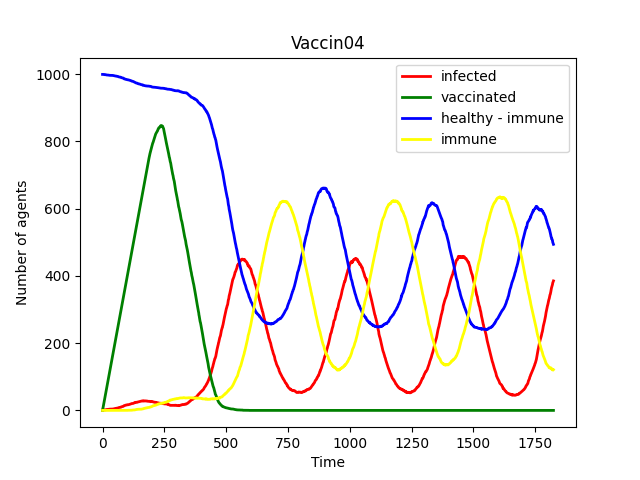
\includegraphics[width=6cm]{../Courbes/1000_agents_1_contaminé_5_ans/Vaccin04.png} }}
	\qquad
	\caption{Représentations graphique de l'évolution de l'état\\ de la population en fonction du nombre de nouveaux vaccinés par jours}

\end{figure}

Ces graphiques montrant l'évolution de l'état de la population en fonction du temps (en jours) pour un nombre de personnes qui se font vacciner chaque jour démontrent bien que
se faire vacciner régulièrement permet de très facilement éradiquer la maladie. En effet, on observe que dès trois personnes vaccinées suplémentaires par jour, la maladie ne dépasse pas les 15\% d'infectés.
Et qu'il suffit de vacciner quatres personnes par jour pour éradiquer la maladie au bout de deux ans.

\subsection{Combinaisons de méthodes}

\end{document}

